This section presents the underlying theory behind some of the methods utilized.

\subsection{Face detection}

Here in this section are the computation of the eye map and mouth map as well as the theory behind the alignment of the faces explained. All of which are methods that are used when deriving the final output of the face detection phase.

\subsubsection{Eye map}
\label{sub:FaceDetection}
Eyes can be located by recognizing signature eye regions in images. One way to due this is through the utilization of the \textit{YCbCr} color space \cite{fdInColorImages}. This process involves the development of a so called \textit{eye map}, which essentially is a gray scale image that is brighter where the locations of the eyes could be present. The eye map itself is derived from two independent components, the \textit{chroma} component and the \textit{luma} component. After these two components have been compiled they are merged via an AND operation to establish the eye map. 

The interesting parts about the YCbCr color space which allows us to proceed this way are that the $C_{b}$ and $C_{r}$ channels are observed to have high variation around the eyes with the addition that eyes most often contain both dark and bright pixels in the Y channel. Because of these observations, as described in \cite{fdInColorImages}, we can construct  the chroma component of the eye map through Equation \ref{eq:eyeMapChroma} and the luma component by Equation \ref{eq:eyeMapLuma}, where $\tilde{C_r}$ is the inverted $C_r$ channel and where $\oplus$ represents the dilation and $\ominus$ the erosion of the $Y$ channel by a kernel $K_{i}$. The kernel $K_{i}$ can be of various shapes, e.g. an ellipse, however in this report is a circular disk used, where the kernel width is proportional to $i$.

\begin{equation} \label{eq:eyeMapChroma}
\begin{split}
eyeMapChroma = \frac{1}{3} \lbrace C_b^2 + \tilde{C_r}^2 + \frac{C_b}{C_r} \rbrace
\end{split}
\end{equation}

\begin{equation} \label{eq:eyeMapLuma}
\begin{split}
  eyeMapLuma = \sum_{i=1}^{10}\frac{Y\oplus K_{i}}{i + Y\ominus  K_{i}}
\end{split}
\end{equation}




% $C_b$ is the blue chroma component and $\tilde{C_r}$ is the inverted $C_r$ $(255 - C_r)$. The terms $C_b^2$, $\tilde{C_r^2}$ and $\frac{C_b}{C_r}$ are normalized to the range $[0, 255]$.

% To estimate the second component, the luminance, we take advantage of the intensity structure area around the eyes in the luminance component, where the pixels are dark and bright. The morphological operations Dilation and Erosion are used with to highlight the area. The kernels are applied iteratively with different size according to Equation \ref{eq:eyeMapLuma}.



% Y is the luminance component, $K_n$ is the kernel with size $n$ and $ n \in [1,10]$. Before the eye maps are combined, the contrast in the eye map chroma component is enhanced by histogram equalization. Finally, the eye maps are combined with the AND operation: $EyeMap = (EyemapC) \textbf{AND} (EyeMapLuma)$. For polarization and better result, facial areas can be suppressed by using dilation and erosion operations. 






% The facial feature detection is an important step to extract a final face mask. As $\cite{fdInColorImages}$ motivates, eyes and mouth are dominant. %features in the research field to perform face detection. ....The maps are estimated in the ycbcr color space
% \newline
% \indent To extract the eyes, two independent eye maps are built. The first is from chrominance components and the second is from luminance components. The two components are then merged with AND-operator to get a final eye mask. The interesting parts in the chrominance component are the red and blue chroma component. These components are observed to have high variation around the eyes for the blue chroma and higher variation for the red chroma component. This observation is important at the choice of the color space. As described in \cite{fdInColorImages}, we construct the eye map of the first component, the chroma component, by Equation $\ref{eq:eyeMapChroma}$
% \begin{equation} \label{eq:eyeMapChroma}
% \begin{split}
% eyeMapChroma = \frac{1}{3} \lbrace C_b^2 + \tilde{C_r^2} + \frac{C_b}{C_r} \rbrace
% \end{split}
% \end{equation}
% , where $C_b$ is the blue chroma component and $\tilde{C_r}$ is negative $C_r$ (255 - $C_r$). The terms $C_b^2$, $\tilde{C_r^2}$ and $\frac{C_b}{C_r}$ are normalized to the range $[0, 255]$.
% \newline
% \newline
% To estimate the second component, the luminance, we take advantage of the intensity structure area around the eyes in the luminance component, where the pixels are dark and bright. The morphological operations Dilation and Erosion are used with to highlight the area.  The kernels are applied iteratively with different size, see Equation $\ref{eq:eyeMapLuma}$
% \begin{equation} \label{eq:eyeMapLuma}
% \begin{split}
%   eyeMapLuma = \sum_{i=1}^{10}\frac{Y\oplus K_{i}}{i + Y\ominus  K_{i}}
% \end{split}
% \end{equation}
% where Y(x,y) is the pixel value in the luminance component, $K_n$ is the kernel with size $n$ and $ n \in [1,10]$.
% \newline
% Before the eye maps are combined, the contrast in the eye map chroma component is enhanced by histogram equalization. Finally, the eye maps are combined with the AND operation: $eyeMap = and(eyeMapChroma, \ eyeMapLuma)$. For polarization and better result, facial areas can be suppressed by using dilation and erosion operations.





\subsubsection{Mouth map}

 As \cite{fdInColorImages} also mentions, the mouth area contain much stronger $C_{r}$ than $C_{b}$ values compared to the other parts of a face. This is due to the fact that the mouth is often more red than blue. By carefully studying combinations of the $C_{r}$ and $C_{b}$ channels one can therefore find out that the mouth region receives a low response by $\frac{C_{r}}{C_{b}}$ and a high response for $C_{r}^2$. As of such it is possible to extract an accurate \textit{mouth map} through Equation \ref{eq:mouthMap} and \ref{eq:nn}.

 % component and weaker blue chrominance component than other areas on the face. We can also observe that the mouth region has strong values for the $C_r^2$ component and low values for the $\frac{C_r}{C_b}$ component. Through this reasoning the mouth map is constructed according to Equation \ref{eq:mouthMap} and \ref{eq:nn}.

\begin{equation} \label{eq:mouthMap}
\begin{split}
mouthMap = C_r^2 \cdot (C_r^2 - \eta \cdot \frac{C_r}{C_b})^2
\end{split}
\end{equation}

\begin{equation} \label{eq:nn}
\begin{split}
\eta = 0.95 \cdot \frac{\frac{1}{n} \cdot \sum\limits_{} C_r^2}{\frac{1}{n} \cdot \sum\limits_{} \frac{C_r}{C_b}}.
\end{split}
\end{equation}

% =======
% As for the chrominance components in the eye map, we can make a similar observations for the colors at the mouth area. As $\cite{fdInColorImages}$ mentions, we can observe that the mouth area contain much stronger red chrominance component and weaker blue chrominance component than other areas on the face. We can also observe that the mouth region has strong values for $C_r^2$ component and low values for $\frac{C_r}{C_b}$ component. The mouth map is therefore designed as
% \newline
% \newline
% \begin{equation}
% MouthMap = (C_r^2 \cdot (C_r^2 - \eta \cdot \frac{C_r}{C_b})^2
% >>>>>>> 05da8faa2dbc6071a6590e65148c469b28a75a03




% \begin{equation} \label{eq:nn}
% \begin{split}
% \eta = 0.95 \cdot \frac{\frac{1}{n} \cdot \sum\limits_{(x,y) \in FG} C_r(x,y)^2}{\frac{1}{n} \cdot \sum\limits_{(x,y) \in FG} \frac{C_r(x,y)}{C_b(x,y)}}.
% \end{split}
% \end{equation}


% $\eta$ is a parameter for the ratio of the average of $C_r^2$ to the average $\frac{C_r}{C_b}$ and $n$ is the number of pixels in the mask. The products $C_r^2$ and $\frac{C_r^2}{C_b^2}$ are normalized to an interval of $[0,255]$. FIGURE!!!!

% =======
% \newline
% Where $\eta$ is a parameter as the ratio of the average of $C_r^2$ to the average $\frac{C_r}{C_b}$ and $n$ is the number of pixels in the mask. The products $C_r^2$ and $\frac{C_r^2}{C_b^2}$ are normalized to an interval of $[0,255]$. FIGURE!!!!
% >>>>>>> 05da8faa2dbc6071a6590e65148c469b28a75a03


\subsubsection{Circular Hough transform}
A compensation for the image plane rotation of a face can be achieved by taking advantage of the symmetry of faces, namely that both eyes most often form a vector that is parallel to the horizontal axis. After the extraction of such a vector, one can easily find the rotation of the face.

The algorithm we use to locate the eyes is called the \textit{Circular Hough Transform} (CHT) which is a feature extraction technique for finding circles. The algorithm is popular and often used because of its robustness in noisy areas and tolerance for occlusion and varying illumination \cite{cht}. However, it does not exits a specific definition of the algorithm steps based on CHT. A brief description of a customized version is included below.

% https://www.cis.rit.edu/class/simg782/lectures/lecture_10/lec782_05_10.pdf

% http://docs.opencv.org/2.4/doc/tutorials/imgproc/imgtrans/hough_circle/hough_circle.html

The first step is locate pixels at regions with high gradient variations. These pixels are called candidate pixels and they have the ability to cast \textit{votes}, in a circular pattern around themselves. An accumulator array is then defined to store the votes. More votes on a pixel increases the likelihood of it being a center point for a circle. The vote-pattern is illustrated by Figure \ref{fig:CHT}.

\begin{figure}[H]
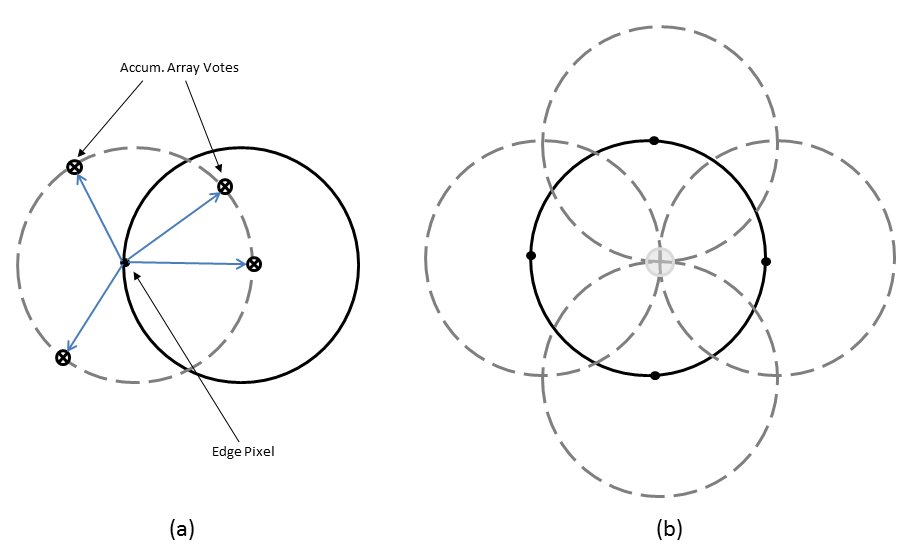
\includegraphics[scale=0.4]{img/fd/accarray.png}
\caption{CHT voting pattern to estimate the center of the circle.}
\label{fig:CHT}
\end{figure}

The second step is to estimate a center point. The position votes from the candidate pixels belonging to an image circle, tend to accumulate at the center of the circle. Therefore, the center of the circle is estimated by detecting the peaks in the accumulator array.




\subsection{Face recognition}
\label{sub:FaceRecognition}
\lipsum[10]


\subsubsection{Eigenfaces}
\label{subs:Eigenfaces}
Eigenfaces can be used as an approach for human face recognition and is the name given to a set of eigenvectors \cite{eigenface1}. According to the authors of \cite{eigenface2} these are the initialization operations to acquire the eigenfaces: 

\begin{itemize}
  \item Prepare a training set of face images.
  \item Calculate the eigenfaces from the training set. Only keep the M images that correspond to the highest eigenvalues. It is these images that defines the \emph{face space}.
  \item Calculate the corresponding distribution in M-dimensional weight space for each known individual and projecting their face images onto the face space. 
\end{itemize}

To calculate the eigenfaces, operations such as matrix multiplication and sums needs to be computed. Firstly we want to subtract the average image from each original image. Let the training set images be $\mathbf{\Gamma}_1,\mathbf{\Gamma}_2,\mathbf{\Gamma}_3...\mathbf{\Gamma}_M $. Also let the average face be $\mathbf{\Psi} $, then each face differs from the average by the vector $\Phi_i=\mathbf{\Gamma}_i - \mathbf{\Psi} $. Secondly we need to calculate the eigenvectors and eigenvalues from the covariance matrix C. This can be done by Equation~\ref{eq:covariance} below. 

\begin{equation}
C = \frac{1}{M}\sum_{n=1}^{M} \mathbf{\Phi}_n \mathbf{\Phi}_n^T = AA^T
\label{eq:covariance}
\end{equation}

Where $A=[\mathbf{\Phi}_1... \mathbf{\Phi}_M]. $ 
	It is possible to determine the eigenvectors of C right away, but it is more efficient to compute the eigenvectors of the smaller matrix $ AA^T $.

The eigenfaces $\mathbf{u}_l $ are given by Equation~\ref{eq:eigenface} below.
\begin{equation}
\mathbf{u}_l = \sum_{k=1}^{M} \mathbf{v}_{lk} \mathbf{\Phi}_k,          l=1...M
\label{eq:eigenface}
\end{equation}
	
	For the face recognition part we need to project a image $\mathbf{\Gamma} $ to the face space $\mathbf{\Omega} = \widehat{U}^T(\mathbf{\Gamma} - \mathbf{\Psi}) $ and determine which face class that image belongs to. Here $\widehat{U}$ is the set of eigenvectors and $\mathbf{\Omega}$ is the weight vector that represents the new face in face space. By minimizing the Euclidean distance which is shown in Equation ~\ref{eq:euclidean} we can determine which face class a certain image belongs to.
	
\begin{equation}
\epsilon_k = \left \| \mathbf{\Omega} - \mathbf{\Omega}_k  \right \| 	
\label{eq:euclidean}
\end{equation}

	In Equation ~\ref{eq:euclidean}, $\mathbf{\Omega}_k$ is a weight vector that represents the \emph{k}th face class. If the distance $\epsilon_k$ is lower than a certain threshold $\mathbf{\Theta} $ the image is considered to belong to the database.

In Figure \ref{fig:eigenface} below some eigenfaces are shown with our implementation.

\begin{figure}[H]
\centering

\begin{subfigure}{.24\textwidth}
  \centering
  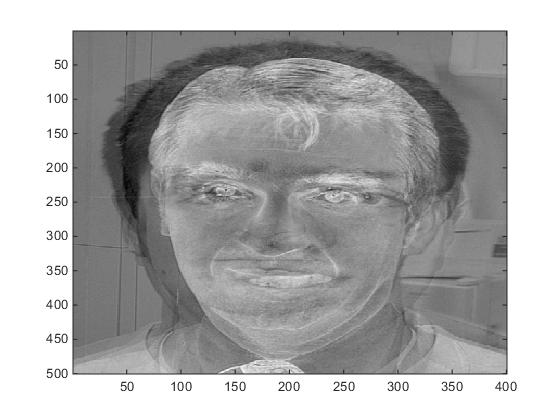
\includegraphics[width=0.95\textwidth]{img/fr/eigenface1.jpg}
  \caption{}
  % \label{fig:sub1}
\end{subfigure}%
\begin{subfigure}{.24\textwidth}
  \centering
  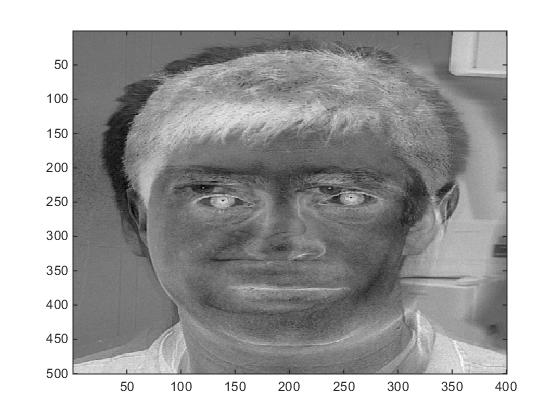
\includegraphics[width=0.95\textwidth]{img/fr/eigenface2.jpg}
  \caption{}
  % \label{fig:sub1}
\end{subfigure}%
\begin{subfigure}{.24\textwidth}
  \centering
  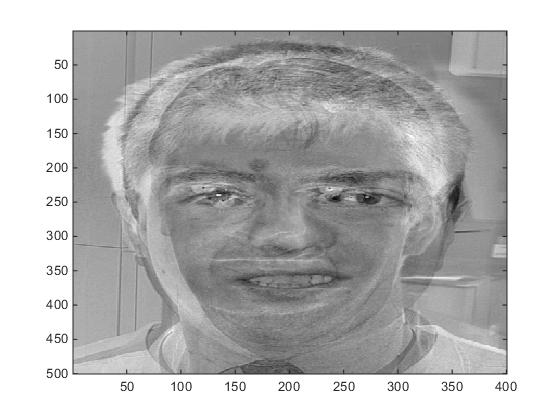
\includegraphics[width=0.95\textwidth]{img/fr/eigenface3.jpg}
  \caption{}
  % \label{fig:sub1}
\end{subfigure}%

\begin{subfigure}{.24\textwidth}
  \centering
  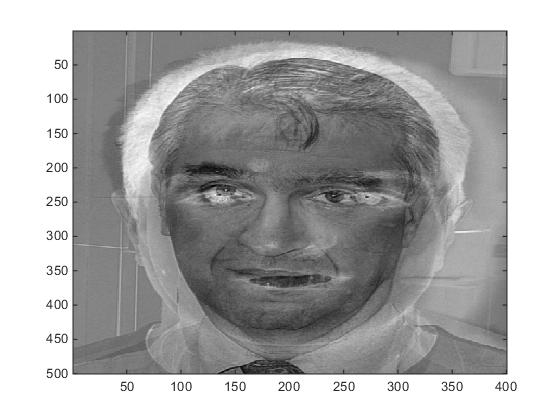
\includegraphics[width=0.95\textwidth]{img/fr/eigenface4.jpg}
  \caption{}
  % \label{fig:sub1}
\end{subfigure}%

\caption{Example of some eigenfaces from our database}
\label{fig:eigenface}
\end{figure}


\subsubsection{Local phase quantization}
\label{subs:LocalPhaseQuantization}
Applying the method of local phase quantization (LPQ) to solve the problem of face recognition was introduced in~\cite{LPQ:1996}. This method is proposed especially to solve the problem of recognizing faces in blurred images since the image descriptions provided by LPQ are considered to be blur invariant.

The LPQ method work under the assumption that the blur in an image can be represented as a function called the point spread function (PSF). The final blurred image can then be obtained by applying a convolution between the clean image and the PSF as seen in Equation~\ref{eq:PSFConv} where where \(i\) is the clean image, \(b\) is the PSF and \(f\) is the blurred image.

\begin{equation}
  f = i \ast b
\label{eq:PSFConv}
\end{equation}

Applying the Fourier transform to Equation~\ref{eq:PSFConv} will result in Equation~\ref{eq:PSFFT} where \(I\), \(B\) and \(F\) represent the Fourier transforms of \(i\), \(b\) and \(f\).

\begin{equation}
  F = I \cdot B
\label{eq:PSFFT}
\end{equation}

Taking the argument of \(F\) in order to compute the phase will result in Equation~\ref{eq:PSFFTPhase} where \(\angle F\), \(\angle I\) and \(\angle B\) is the phase of \(F\), \(I\) and \(B\) respectively.

\begin{equation}
  \angle F = \angle I \cdot \angle B
\label{eq:PSFFTPhase}
\end{equation}

From Equation~\ref{eq:PSFFTPhase} a blur invariant descriptor of the image can be derived using two properties of the Fourier transform. The first is the property that states that the Fourier transform of a symmetric function will be a real value function~\cite[p. 151]{FandLTransforms}. By combining this with the knowledge from~\cite{PSFSymmetry} that PSFs are generally symmetric and that the phase of a real value function is either \(0\) or \(\pi\) the conclusion can be reached that \(\angle B\) can only assume the values \(0\) or \(\pi\). Further more~\cite{LPQ:1996} claims that regular PSFs are often close in shape to a Gaussian or a sinc function which as shown in~\cite[p. 144-148]{FandLTransforms} have a positive Fourier transform for small enough frequencies. This realization leads to the conclusion that \(\angle B = 0\). Using this in Equation~\ref{eq:PSFFTPhase} results in Equation~\ref{eq:PSFFTFinal} that indicates that \(\angle F\) is a blur invariant descriptor of the image since it is not dependent on the PSF.

\begin{equation}
  \angle F = \angle I
\label{eq:PSFFTFinal}
\end{equation}

In order to compute the phase of the image a short-time Fourier transform (STFT) is used. The STFT computes the Fourier transform for a given frequency interval that is chosen to be small enough for \(B > 0\) to be valid. Four such intervals, seen in Equation~\ref{eq:LPQIntervals}, are chosen and computed per pixel.

\begin{equation}
  u_{1} = \left [ a, 0 \right ], u_{2} = \left [ 0, a \right ], u_{3} = \left [ a, a \right ], u_{4} = \left [ a, -a \right ]
\label{eq:LPQIntervals}
\end{equation}

For every pixel the real and imaginary parts of each STFT computation is stored separately and transformed into a binary representation using Equation~\ref{eq:LPQBinary}.

\begin{equation}
  g = \begin{Bmatrix}
   1, & if\ g \geq 0\\
   0, & else
  \end{Bmatrix}
\label{eq:LPQBinary}
\end{equation}

Combining the binary representations of the real and imaginary parts of all four STFT values results in an 8-bit binary value that can be transformed into a decimal number between \(0\) and \(255\). Finally the image descriptor can be derived by computing a histogram over the decimal numbers representing each pixel.

Once the image descriptor have been computed it can be compared with other descriptors to see if their respective images can be considered a match. The comparison is performed by calculating the average euclidean distance between the values in the descriptors. If the distance is smaller than a certain threshold the images are considered a match.

